\section{St Anthony and Practical Reason}
\label{sec:St Anthony and Practical Reason}

\begin{wrapfigure}{rt}{.35\textwidth}
 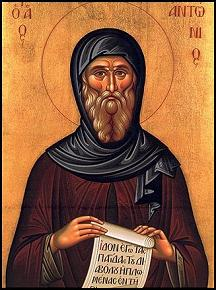
\includegraphics[scale=.6]{a20100530StAnthonyandPracticalReason-img001.jpg} 
\end{wrapfigure}

What follows are some of the main themes of \textbf{St Anthony}`s “Counsels on the Character of Men and on
the Virtuous Life”, from the \textit{Philokalia}, Volume I, translated by \textbf{Constantine Cavarnos}. Dr. Cavarnos includes
copious footnotes relating St Anthony's essay to biblical passages, apparently to counteract the claims of
the first translators, which we have previously documented\footnote{\url{https://www.gornahoor.net/?p=497}}. Nevertheless, it is unlikely you will hear these themes in
a Sunday sermon, or from a TV preacher.

\paragraph{Practical Reason}
\begin{quotex}
Men are improperly called rational; it is not those who have learned thoroughly the discourses and books of the wise men
of old that are rational, but those who have a rational soul and can discern what is good and what is evil, and avoid
what is evil and harmful to the soul, but zealously keep, with the aid of practice, what is good and beneficial to the
soul … 

\end{quotex}
The “book learning” St Anthony refers to may be called “theoretical reason”. But what makes a man truly rational is the
“practical reason”, that is, the ability to choose ones ends or goals and the means to achieve them. Since man is the
“rational animal”, someone who does not possess practical reason is really “inhuman”, being more like the irrational
animals.

\begin{quotex}
Just as helmsmen steer the ship in the proper direction in order to avoid hitting a reef or shoal, so let those who
aspire after the virtuous life consider carefully what they ought to do and what they ought to avoid. 

\end{quotex}
\paragraph{Freedom}
Those who “are free in their life and ways”, are properly called free. 

\begin{quotex}
Freedom and happiness of the soul consist in genuine purity and contempt of transitory things.

\end{quotex}
\paragraph{Characteristics}
\begin{quotex}
A truly rational and virtuous soul is recognized from a man's look, walk, voice, laughter, manner of
spending his time, and the circumstances of his life. Everything in such a soul has been thoroughly changed and
corrected so as to become graceful. 

\end{quotex}
A virtuous life is like a work of art, with the soul as artist: 

\begin{quotex}
Like skilled painters and sculptors, it is by their works that they display their virtuous and God-loving way of life.

\end{quotex}
\paragraph{Rulers}
\begin{quotex}
Examine the things that pertain to you, and prove for yourself that rulers and masters have authority only over the
body, not over the soul; and let this always be before your mind. 

\end{quotex}
This is even more important in our day when propaganda has become a science. Pay attention to the sources of your
concepts and values to determine if they are truly good, or simply absorbed from the mass media.

\paragraph{Vigilance}
The soul's “God-loving rational faculty, being a vigilant gatekeeper, bars entry to evil and ugly thoughts.”
We are accustomed to regarding thoughts as our own, without considering the source. We are bombarded by thoughts\footnote{\url{https://www.gornahoor.net/?p=451}}; they
are the key to influencing our behavior. A man must be the detached observer of his thoughts, paying attention to their
origin\footnote{\url{https://www.gornahoor.net/?p=309}}, before latching onto a thought and letting it guide his actions.

\paragraph{Obstacles}
St Anthony lists many obstacles to a virtuous life. Again, the point is not to be “good” in order to get a reward, but
rather to recognize those attitudes that prevent us from leading the rational life. The spirit [\emph{nous}, mind] must
guide the soul which masters the body. The “passions”, on the other hand, make us passive, not the active agent\footnote{\url{https://www.gornahoor.net/?p=203}} of our
life. In one place he lists “lust, love of glory, and ignorance”. In another, “conceit, arrogance, deception, envy,
avarice”. The point is that these temptations tie us to transitory things, dominate the soul, and thus prevent our full
use of reason and freedom.

\paragraph{Many paths}
\begin{quotex}
Through God's love for man, there are many paths that lead men to salvation, ways that convert men and lead
them to the Heavens. 

\end{quotex}

\flright{\itshape Posted on 2010-05-30 by Cologero}
